\documentclass[aspectratio=169,smaller]{beamer}%,handout



\newcommand\hmmax{0}
\newcommand\bmmax{0}

%======================================================================================================
%
% BEAMER PACKAGES FILE (A. FIORUCCI)
% AFFILIATION : ECOLE POLYTECHNIQUE
%
%======================================================================================================

%======================================================================================================
% LATEX PACKAGES
%======================================================================================================

% Typesetting packages
	\usefonttheme{professionalfonts}
	\usepackage[UKenglish]{babel}
	\usepackage[T1]{fontenc}
	\usepackage{libertine}
	\usepackage[libertine]{newtxmath}
	\usepackage[cal=euler,scr=boondoxo]{mathalfa}
		
%% Math and symbols
	\usepackage{amssymb}
	\usepackage{amsmath}
	\usepackage{amsfonts}
	\usepackage{mathtools}
	\usepackage{bm}
	\usepackage{upgreek}
	\usepackage{cancel}
	\usepackage{fontawesome}
	\usepackage{wasysym}
	\usepackage{bigints}
	\usepackage{slashed}
	
% Layout
	\usepackage[absolute,overlay]{textpos}
	\usepackage{graphicx}
	\usepackage{float}
	\usepackage{graphbox}
	
% Tikz drawings
	\usepackage{xcolor}
	\usepackage{tikz}
	\usetikzlibrary{calc}
	\usetikzlibrary{decorations.pathreplacing}
	\usetikzlibrary{decorations.pathmorphing}
	\usetikzlibrary{decorations.markings}
	\usetikzlibrary{arrows.meta}
	\usetikzlibrary{positioning}
	\usetikzlibrary{shadows,shadings}
	\usepackage{tikzsymbols}
	\usepackage{pgf-pie}
	
% Arrays
	\usepackage{array}
	\newcolumntype{C}[1]{>{\centering\let\newline\\\arraybackslash\hspace{0pt}}m{#1}}	
	
% Page format
	\usepackage[toc,page]{appendix}
	\usepackage{caption}
	\usepackage{changepage}
	\usepackage{setspace}
	\usepackage[labelformat=simple]{subfig}
	\renewcommand{\thesubfigure}{\relax}
	\usepackage[export]{adjustbox}
	\usepackage{appendixnumberbeamer}
	\usepackage{multirow}

% Multimedia content
	\usepackage{multimedia}
	
% References
	\usepackage{hyperref}

	\usepackage{comment}
	
%======================================================================================================
% BEAMER SPECIFIC SETTINGS
%======================================================================================================

% Define institute colors
	\definecolor{xblue}{RGB}{1,66,106}
	\definecolor{xlightblue}{RGB}{184,211,225}
	\definecolor{xgray}{RGB}{150,150,150}
	\definecolor{xsepia}{RGB}{166,139,78}
	\definecolor{xred}{RGB}{200,32,33} %{169,32,33}
	\definecolor{xorange}{RGB}{254,80,0}
	\definecolor{xgreen}{RGB}{67,176,42}
	\definecolor{xpurple}{RGB}{77,22,84}
	\definecolor{xpink}{RGB}{227,28,121}

% Main theme
	\usetheme{Madrid}
	\setbeamersize{text margin left=20pt,text margin right=20pt} 

% Main colour
	\usecolortheme[named=xblue]{structure}

% Layout of the slide
	\setbeamertemplate{navigation symbols}{} % No navigation symbol at the bottom of the page
	\setbeamercolor{frametitle}{fg=xblue,bg=gray!20}
	\setbeamerfont{frametitle}{family=\rmfamily,shape=\scshape}
	
% Layout of the blocks
\setbeamercolor{block title}{fg=xblue,bg=gray!20}
	\setbeamerfont{block title}{family=\rmfamily,shape=\scshape}


% Item bullets
	\setbeamertemplate{enumerate items}[square]
	\setbeamertemplate{sections/subsections in toc}[square]
	
\newcommand{\sectionframe}{
\begingroup
\setbeamercolor{page number in head/foot}{fg=xblue}
\begin{frame}{Outline of the talk}
	\tableofcontents[currentsection]
\end{frame}
\endgroup
\addtocounter{framenumber}{-1}
}

%======================================================================================================
% PERSONAL COMMANDS
%======================================================================================================

\usepackage{appendixnumberbeamer}
\newcommand{\backupbegin}{
   \newcounter{framenumberappendix}
   \setcounter{framenumberappendix}{\value{framenumber}}
}
\newcommand{\backupend}{
   \addtocounter{framenumberappendix}{-\value{framenumber}}
   \addtocounter{framenumber}{\value{framenumberappendix}} 
}

% Custom colours
	\definecolor{darkred}{RGB}{192,0,0} 
	\definecolor{Cgreen}{RGB}{0,153,0}
	\definecolor{oldbook}{RGB}{255,222,117}

% Custom symbols
	\newcommand{\D}{\text{d}}
	\newcommand{\indep}{\raisebox{0.05em}{\rotatebox[origin=c]{90}{$\models$}}}
	\newcommand{\ndelta}{\delta\hspace{-0.50em}\slash\hspace{-0.05em} }

% Semi-direct sum
	\usepackage{pict2e}
	\makeatletter
		\newcommand{\loplus}{\mathbin{\mathpalette\dog@lsemi{+}}}
		\newcommand{\dog@lsemi}[2]{\dog@semi{#1}{#2}{270,90}}
		\newcommand{\dog@semi}[3]{%
  		\begingroup
  			\sbox\z@{$\m@th#1#2$}%
  			\setlength{\unitlength}{\dimexpr\ht\z@+\dp\z@\relax}%
  			\makebox[\wd\z@]{\raisebox{-\dp\z@}{%
    		\begin{picture}(1,1)
    			\linethickness{\variable@rule{#1}}
    			\roundcap
    			\put(0.5,0.5){\makebox(0,0){\raisebox{\dp\z@}{$\m@th#1#2$}}}
    			\put(0.5,0.5){\arc[#3]{0.5}}
    		\end{picture}%
  		}}%
  		\endgroup
		}
		\newcommand{\variable@rule}[1]{%
 		\fontdimen8  
  		\ifx#1\displaystyle\textfont3\else
    	\ifx#1\textstyle\textfont3\else
      	\ifx#1\scriptstyle\scriptfont3\else
        \scriptscriptfont3\relax
  		\fi\fi\fi
		}
	\makeatother

% Text article references
	\newcommand{\cit}[1]{{\footnotesize \color{xsepia} \normalfont{[#1]}}}
% Text talks
	\newcommand{\cittalk}[1]{{\footnotesize \color{xorange} \normalfont{[#1]}}}
	
% Small quotations
	\newcommand{\quot}[1]{{\footnotesize \color{gray} \normalfont{#1}}}
		
% Important results
	\usepackage{mdframed}
	\global\mdfdefinestyle{HL}{
		linecolor=xblue, linewidth=1pt,%
		topline=false, bottomline=false, rightline=false,%
		align=left, backgroundcolor=xblue!20, userdefinedwidth=\textwidth,%
		innerleftmargin=5, innertopmargin=5, innerbottommargin=5, innerrightmargin=5, skipabove=5}
		
	\global\mdfdefinestyle{HLrelax}{
		linecolor=xblue, linewidth=1pt,%
		topline=false, bottomline=false, rightline=false,%
		align=left, backgroundcolor=xblue!20,%
		innerleftmargin=5, innertopmargin=5, innerbottommargin=5, innerrightmargin=5, skipabove=5}

	\newcommand{\hl}[1]{
		\begin{mdframed}[style=HL]
		#1
		\end{mdframed}
		\vspace{8pt}
	}
	
	\newcommand{\hlrelax}[1]{
		\begin{mdframed}[style=HLrelax]
		#1
		\end{mdframed}
		\vspace{8pt}
	}

	
%======================================================================================================

% PERSONAL COMMANDS
\newcommand{\bfupsilon}{{\bm{\upupsilon}}}
\newcommand{\bfxi}{{\bm{\upxi}}}
\newcommand{\bfg}{{\text{\bf g}}}
\newcommand{\bfd}{{\bm\partial}}
\newcommand{\hframe}{{\text{\bf e}}}
\newcommand{\htheta}{{\bm{\uptheta}}}
\newcommand{\bftau}{{\bm\uptau}}
\newcommand{\bfomega}{{\bm\upomega}}
\newcommand{\bfG}{{\text{\bf G}}}
\newcommand{\bfmu}{\bm{\upmu}}
\newcommand{\vect}[1]{{\text{\bf #1}}}
\newcommand{\pd}[3][]{\dfrac{\partial^{#1}#2}{\partial #3}}     % partial derivative: \pd[n]{f}{x}
\newcommand{\kB}{k_\mathrm{B}}
\newcommand{\bigO}[1]{\mathcal{O}\!\left(#1\right)}
\newcommand*\diff{\mathop{}\!\mathrm{d}}

\newcommand{\C}{\mathrm{C}}

\newcommand{\highlight}[1]{%
  \colorbox{red!40}{$\displaystyle#1$}}

% Allow a custom "reference" field for the title frame.  frontframe.tex
% uses \insertreference, so provide a default and a setter.
\providecommand{\insertreference}{}
\newcommand{\reference}[1]{\gdef\insertreference{#1}}

%======================================================================================================
% TITLE PAGE SETTINGS
%======================================================================================================

\title[Quantum cosmology and Liouville theory]{\textbf{Quantum cosmology, Euclidean wormholes and Liouville theory}}
\author[P. Ghiringhelli]{Paul \textsc{Ghiringhelli}} 
\institute[CPHT École polytechnique]{École polytechnique, Centre de Physique Théorique (CPHT)}
\reference{Based on \cit{2602.23432} with P.\ Betzios, O.\ Papadoulaki, I.\ Gialamas \\ and on works to appear with P.\ Betzios, O.\ Papadoulaki, I.\ Tsiares}

\date{23 September 2026}
\subtitle{CSI}

%======================================================================================================
% BEGIN SLIDESHOW
%======================================================================================================

\begin{document}

%======================================================================================================
% TITLEPAGE
%======================================================================================================

\begingroup
% Remove header and footline
\setbeamertemplate{headline}{}
\setbeamertemplate{footline}{}
% Plain frame
\begin{frame}[plain]

\begin{tikzpicture}[remember picture,overlay]
    % Outer frame
    \draw [draw=xlightblue,thick] ($(current page.north west)+(.3,-.3)$) rectangle ($(current page.south east)+(-.3,.3)$);
    % Title
    \node[align=center,text width=0.9\textwidth,inner sep=0.3cm] (title) at ($(current page.center)!0.65!(current page.north)$) {{\Large \color{xblue} \sc \inserttitle}};
    % Author
	 \node[align=center,black] (author) at ($(title)-(0,40pt)$) {\bfseries\insertauthor};
	 % Institute
	 \node[align=center,black] (institute) at ($(author)-(0,30pt)$) {\small\insertinstitute};
	 % Location
	 \node[align=center,black] (location) at ($(institute)-(0,30pt)$) {\small\bfseries\insertsubtitle};
	 % Reference
	 \node[align=center,black] (reference) at ($(location)-(0,45pt)$) {\small\insertreference};
	 % Date
	 \node[align=center,black,below,yshift=-5pt] (date) at (location) {\small\insertdate};
	 % Institution logo
	 \node[anchor=south west] (llogo) at ($(current page.south west)+(.5,.5)$) {
\includegraphics[height=1.2cm]{RVB}};
	 \node[anchor=south] (clogo) at ($(current page.south)+(0,.5)$) {
\includegraphics[height=1.2cm]{cnrs}};
%	 \node[] (mlogo) at ($(llogo)!0.5!(clogo)$) {
\includegraphics[height=.9cm]{cnrs}};
	 \node[anchor=south east] (rlogo) at ($(current page.south east)+(-.5,.5)$) {
\includegraphics[height=1.2cm]{cpht}};
\end{tikzpicture}
\addtocounter{framenumber}{-1}
\end{frame}
%
%
%
%\begin{frame}[plain]
%
%\begin{tikzpicture}[remember picture,overlay]
%    % Outer frame
%    \draw [draw=xlightblue,thick] ($(current page.north west)+(.3,-.3)$) rectangle ($(current page.south east)+(-.3,.3)$);
%\end{tikzpicture}
%
%\begin{center}
%    \textsc{Based on}\\[4pt]
%	A. Fiorucci, S. Pekar, P. M. Petropoulos and M. Vilatte,\\[4pt] {\bfseries \color{xblue} Carrollian-holographic Derivation of \\ Gravitational Flux-balance Laws}\\[4pt]
%	Phys. Rev. Lett. \textbf{135} (2025) 26, 261602\\[2pt]
%	\texttt{[arXiv:2505.00077]}	\\[5pt]
%	
%	\bigskip
%	\bigskip
%	
%	\textsc{Work supported by}\\[2pt]
%	\textbf{Centre National de la Recherche Scientifique} (France) \\
%	\textbf{Fondation de l'École polytechnique} (France) \\
%	\textbf{Solvay Fund granted to Prof. Henneaux} (Belgium)
%\end{center}
%
%\addtocounter{framenumber}{-1}
%\end{frame}
\endgroup

\begin{frame}{Plan}
  \begin{columns}[T]
    \begin{column}{0.48\textwidth}
      \textbf{I. Wineglass cosmology and wormholes}
      \begin{itemize}
        \item No-boundary instantons
        \item Wineglass Euclidean preparation
        \item Phase diagram of saddles
        \item Cosmological correlators
      \end{itemize}
    \end{column}
    \begin{column}{0.48\textwidth}
      \textbf{II. Boundary Liouville theory}
      \begin{itemize}
        \item Spacelike vs timelike regimes
        \item Boundary bootstrap data
        \item Moore--Seiberg consistency
        \item Preliminary timelike results
      \end{itemize}
    \end{column}
  \end{columns}
\end{frame}

\section{Wineglass wormholes and cosmology}

\begin{frame}[plain]
  \centering
  {\Large\textbf{Part I --- Wineglass cosmology and wormholes}}\\[0.6cm]
\end{frame}

\begin{frame}{No-boundary instantons and the wavefunction of the universe}
	\vspace{-0.3cm}
	\begin{block}{Minisuperspace saddle point problem}
		\begin{equation*}
		\begin{aligned}
			\mathcal{S}_E &= -\frac{1}{2}\int \rm{d}^4 x \sqrt{g_E}\left(\frac{\mathcal{R}}{2\kappa}+ \Lambda\right) + \mathcal{S}_{\rm GHY}\,, \quad \kappa = 8\pi G_N\,.\\
			\rm{d}s^2 &= \rm{d}\tau^2 + a^2(\tau) \rm{d}\Omega_3^2 \Rightarrow a(\tau) = \frac{\cos(H\tau)}{H}\,, \quad \Lambda = 3H^2\,.
		\end{aligned}
		\end{equation*}
		Four "complex" regular saddles with $a(\tau_i)=0,\, a(\tau_f=b)$
		\vspace{-0.2cm}
		\begin{equation*}
    i\mathcal{S}_L^{(\sigma,\eta)}
    =\sigma\,\frac{4\pi^2}{\kappa H^2}
    \left[
        1-\eta\,i\big((bH)^2-1\big)^{3/2}
    \right]\,,
    \qquad \sigma,\eta=\pm1\,.
	\end{equation*}
	\end{block}
	\vspace{-0.2cm}
	\begin{figure}[h!]
		\centering
		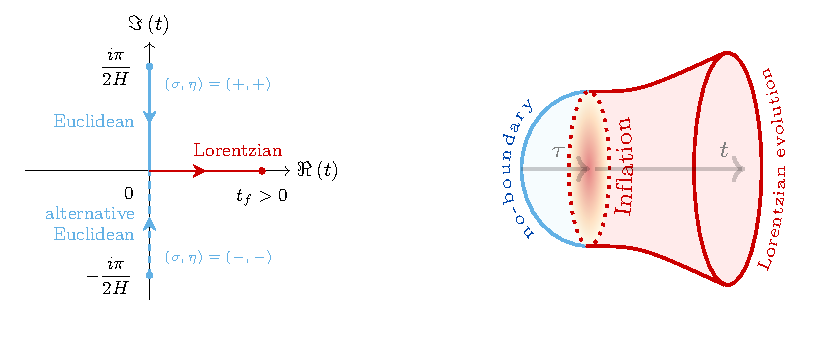
\includegraphics[width=0.65\textwidth]{Figures_Oral_CSI/noboundinstantons.pdf}
	\end{figure}
\end{frame}

\begin{frame}{Hartle-Hawking vs Vilenkin proposal in single-field slow-roll inflation}
	\begin{block}{Single-field minisuperspace slow-roll}
		Scalar field minimally coupled to gravity with slow-roll potential $V(\phi)\sim \Lambda=3H^2$.
	\end{block}
		\vspace{-0.15cm}
	\pause
	\begin{columns}
		\begin{column}{0.49\textwidth}
				\begin{block}{}
					\textbf{Hartle-Hawking}
					\begin{itemize}
						\item 2 instantons
						\item $\Psi_{\rm HH}(a,\tilde{\phi}) $ \begin{equation*}
						\propto \exp\left[{\color{red}+}\frac{4\pi^2}{\kappa \tilde{V}}\right]\cos\left[\frac{4\pi^2}{\kappa \tilde{V}}((a \tilde{V})^2-1)^{3/2}-\frac{\pi}{4}\right]\,.
					\end{equation*}
					\item $\color{red}+$ sign in the exponent $\Rightarrow$ \textbf{enhanced probability for small $\tilde{V}$} $\Rightarrow$ \textbf{small number of e-folds}.
					\item (But good behavior under perturbations $t = {\color{red}-}i \tau$)
					\end{itemize}
				\end{block}
		\end{column}
		\pause
		\begin{column}{0.45\textwidth}
				\begin{block}{}
					\textbf{Vilenkin (Tunneling)}
					\begin{itemize}
						\item 1 "outgoing" instanton
						\item $\Psi_{\rm T}(a,\tilde{\phi}) $ \begin{equation*}
						\propto \exp\left[{\color{blue}-}\frac{4\pi^2}{\kappa \tilde{V}}\left(1+i\left((a\tilde{V})^2-1\right)^{3/2}\right)\right]\,.
					\end{equation*}
					\item $\color{blue}-$ sign in the exponent $\Rightarrow$ \textbf{enhanced probability for large $\tilde{V}$} $\Rightarrow$ \textbf{large number of e-folds}.
					\item (But bad behavior under perturbations $t = {\color{blue}+}i\tau$)
					\end{itemize}
				\end{block}
			
		\end{column}
	\end{columns}
\end{frame}

\begin{frame}{Wineglass Ideology}
	\textbf{Goal: keep the good perturbative behavior while avoiding the unwanted weighting.} \\
	\begin{block}{Basic mechanism}
   HH gives $\Psi\sim e^{-\mathcal{S}_E}$.  Can a negative-potential Euclidean region reverse the problematic weighting?
    \end{block}
	\pause
	\begin{columns}
		\begin{column}{0.49\textwidth}
			\begin{block}{}
				\begin{itemize}
					\item Euclidean solutions are asymptotically EAdS.
					\item Solutions of interest need to be $\mathbb{Z}_2$ symmetric and present a local maximum $\Rightarrow$ Wineglass Euclidean wormholes.
					\item Spherical wormholes require negative Euclidean energy density.
				\end{itemize}
			\end{block}
		\end{column}
		\begin{column}{0.49\textwidth}
				\begin{figure}[h!]
			\centering
			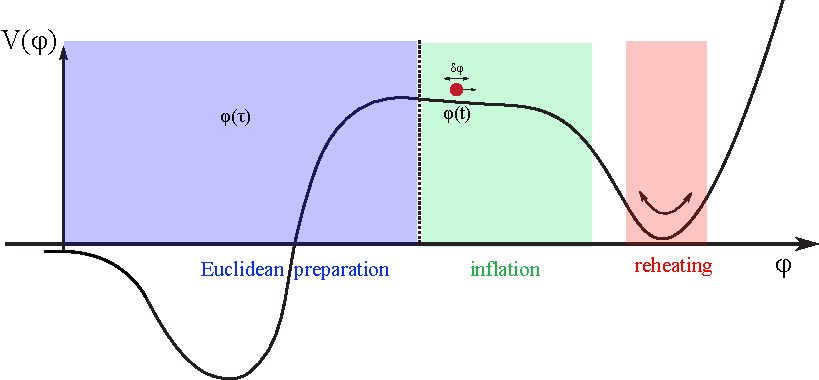
\includegraphics[width=0.9\textwidth]{Figures_Oral_CSI/PotentialHistory.pdf}
		\end{figure}
		\end{column}
	\end{columns}

\end{frame}

\begin{frame}{Concrete realization in Einstein+scalar+$U(1)^3$ theory}
	\begin{block}{}
	\begin{equation*}
	\begin{aligned}
		\mathcal{S}_E &= \int {\rm d}^4x \sqrt{g_E} \left(-\frac{\mathcal{R}}{2\kappa} + \frac12 (\partial_\mu\phi)^2 +V(\phi) + \frac{1}{4}F_{\mu \nu}^{I} F^{\mu \nu, I} \right)+\mathcal{S}_{\rm GHY}\,.\\
    \rm{d}s^2 &= \rm{d}\tau^2 + a^2(\tau) \rm{d}\Omega_3^2\,, \quad \phi = \phi(\tau)\,, \quad A^{(I)}(\tau) = \omega^{(I)} H(\tau)\,.
	\end{aligned}
	\end{equation*}
	\end{block}
	\begin{columns}
		\begin{column}{0.49\textwidth}
			\begin{block}{}
		\begin{align*}
\tilde{\phi}''+3\frac{a'\tilde{\phi}'}{a}-\frac{{\rm d}\tilde{V}(\tilde{\phi})}{{\rm d} \tilde{\phi}} &= 0\,, 
\\
\frac{a'^2}{a^2} -\frac{1}{a^2}  + \left(\tilde{V}(\tilde{\phi})-\frac{\tilde{\phi}'^2}{2} \right) - \frac{\tilde{\rho}^E_{\rm rad}}{a^4} & =0 \,,
\\
\tilde{\rho}^E_{\rm rad} = 2\kappa a^4 \left[ \left(\frac{H'}{a} \right)^2 - \frac{4H^2}{a^4} \right] & < 0 \,
\,.
\label{eq:eoms_Eucl}
\end{align*}
	\end{block}
		\end{column}
		\pause 
		\begin{column}{0.49\textwidth}
			\begin{block}{}
				\begin{itemize}
					\item \textbf{Background subtraction} was employed.
					\item \textbf{IR condition}: solutions are even. Then $\Rightarrow Z(H_{\rm UV},\phi^{(-)}=0)$.
					\item Analyse both Neumann and Dirichlet BCs for the scalar and the gauge field.
				\end{itemize}
			\end{block}
		\end{column}
	\end{columns}
	

\end{frame}

\begin{frame}{A zoology of Euclidean solutions}
	\vspace{-0.2cm}
	\begin{block}{}
		In practice, for Wineglass running solutions, postulate a scale factor and find the associated potential
				\begin{equation*}
 a_{WG}^2(\tau) = 
    \begin{cases}
   \displaystyle   \frac{1}{4 H_{\rm I}^2\cosh(\bar{\tau}^{\textbf{I}})}\left(\sqrt{A_{\rm I}}\cosh{(\bar{\tau}^{\textbf{I}})}-\frac{1}{\sqrt{A_{I}}}\right)^2\,, \bar{\tau}^{\textbf{I}} = 2H_{\rm I} (\tau-\tau_{\rm min})<0\,. \quad (\textbf{I}) &  
\\[0.3cm]
   \displaystyle     \frac{1}{4 H_{\rm II}^2} \left(\cos{(\bar{\tau}^{\textbf{II}})}- 16 \tilde{\rho}^E_{\rm rad} H_{\rm II}^2-1\right)\,, 2H_{\rm II}\tau_{\rm min}<\bar{\tau}^{\textbf{II}} = 2H_{\rm II}\tau <0\,.  \hspace{1.2cm} (\textbf{II}) &
\end{cases}
\label{eq:background_ans_simple}
\end{equation*}
			\end{block}
	\vspace{-0.15cm}
	\pause
	\begin{columns}
		\begin{column}{0.27\textwidth}
			\centering
			\textbf{Disconnected, non-running and}  $F = \star F$\\
			\vspace{1.3cm}
			\textbf{Running Wineglass $\phi(\tau)$ and $\tilde{\rho}^{E}_{\rm rad}<0$}
		\end{column}
		\begin{column}{0.39\textwidth}
			\begin{figure}[h!]
		\centering
		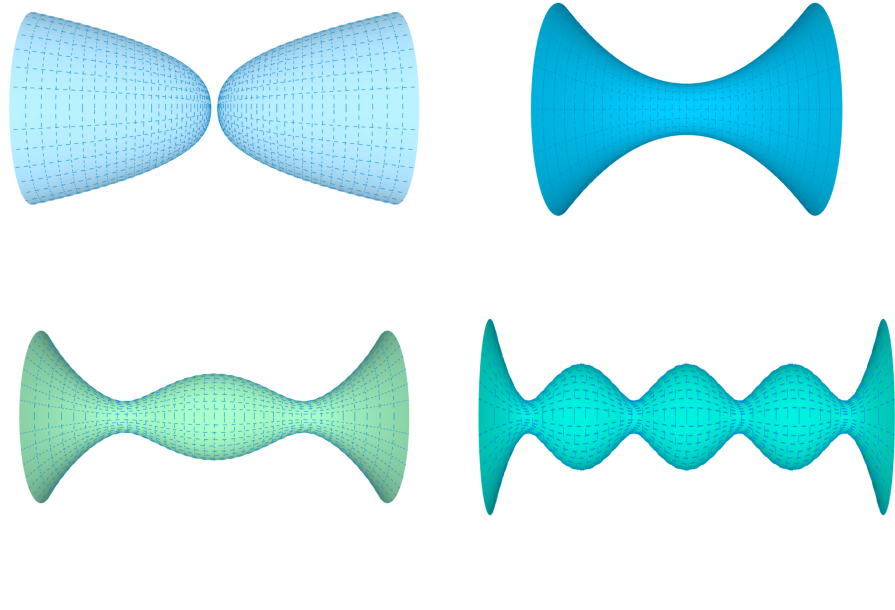
\includegraphics[width=1\textwidth]{Figures_Oral_CSI/wormall.pdf}
		
		\end{figure}
		\end{column}
		\begin{column}{0.27\textwidth}
			\centering
			\textbf{Non-running wormhole} and  $\tilde{\rho}^{E}_{\rm rad}<0$\\
			\vspace{1.3cm}
			\textbf{Oscillatory Wineglass}
		\end{column}
	\end{columns}
\end{frame}

\begin{frame}{Results: diagram of dominance}
	\begin{columns}
		\begin{column}{0.39\textwidth}
			\begin{itemize}
				\item Solutions are compared with the same sources at the EAdS boundary.
				\item Scalar field characterised by $\Delta_+ = 2,\, \Delta _- = 1$. Scalar field source set to zero to compare with non-running solutions.
				\item \textbf{Energy density is an IR parameter! $\tilde{\rho}^E_{\rm rad} = - 8 \kappa H^2_{0}$}.
			\end{itemize}
		\end{column}
		\begin{column}{0.59\textwidth}
			\begin{figure}[h!]
				\centering
			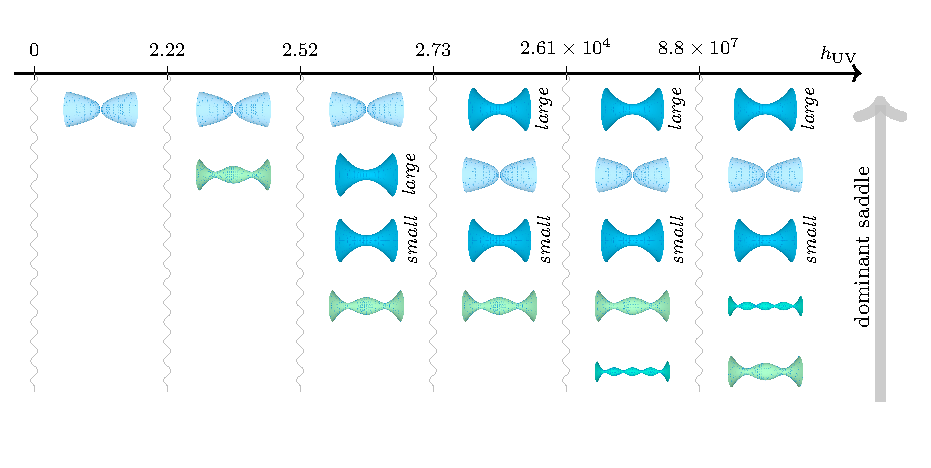
\includegraphics[width=1\textwidth]{Figures_Oral_CSI/Neumannphasediagram.pdf}
			\caption{Diagram of dominance with Neumann boundary conditions for the scalar field and Dirichlet boundary conditions for the gauge field.}
			\end{figure}
		\end{column}
	\end{columns}
\end{frame}

\begin{frame}{Cosmological correlators: massless scalar probe in a fixed background}
	\begin{block}{}
		Massless scalar probe on top of the background (QFT in curved spacetime)
		\begin{equation*}
		\begin{aligned}
			\mathcal{S}_{\Phi} &= -\frac{1}{2}\int \rm{d}^4x \sqrt{-g} \partial_\mu \Phi \partial^\mu \Phi\,, \quad \Phi = \sum Q_{n \ell m}\Phi_{n \ell m}\,.\\
			0&=\ddot{\Phi}_{n \ell m}(t)+3\frac{\dot{a}}{a}\,\dot{\Phi}_{n \ell m}(t)
  	+\frac{n^2-1}{a^2}\Phi_{n \ell m}(t)\,.
		\end{aligned}
		\end{equation*}
	\end{block}
	\vspace{-0.2cm}
	\pause
	\begin{columns}
		\begin{column}{0.49\textwidth}
		\begin{block}{}
			\begin{itemize}
				\item \textbf{Bayesian} question.
				\item For a \textbf{free theory}, $\langle |\Phi_{n \ell m}|^2\rangle$ is obtained from the classical EOM, and the boundary conditions give the vacuum prescription. We impose \textit{Euclidean normalizability} at the EAdS boundary.
			\end{itemize}
		\end{block}
		\end{column}
		\begin{column}{0.49\textwidth}
			\begin{figure}[h!]
			\centering
			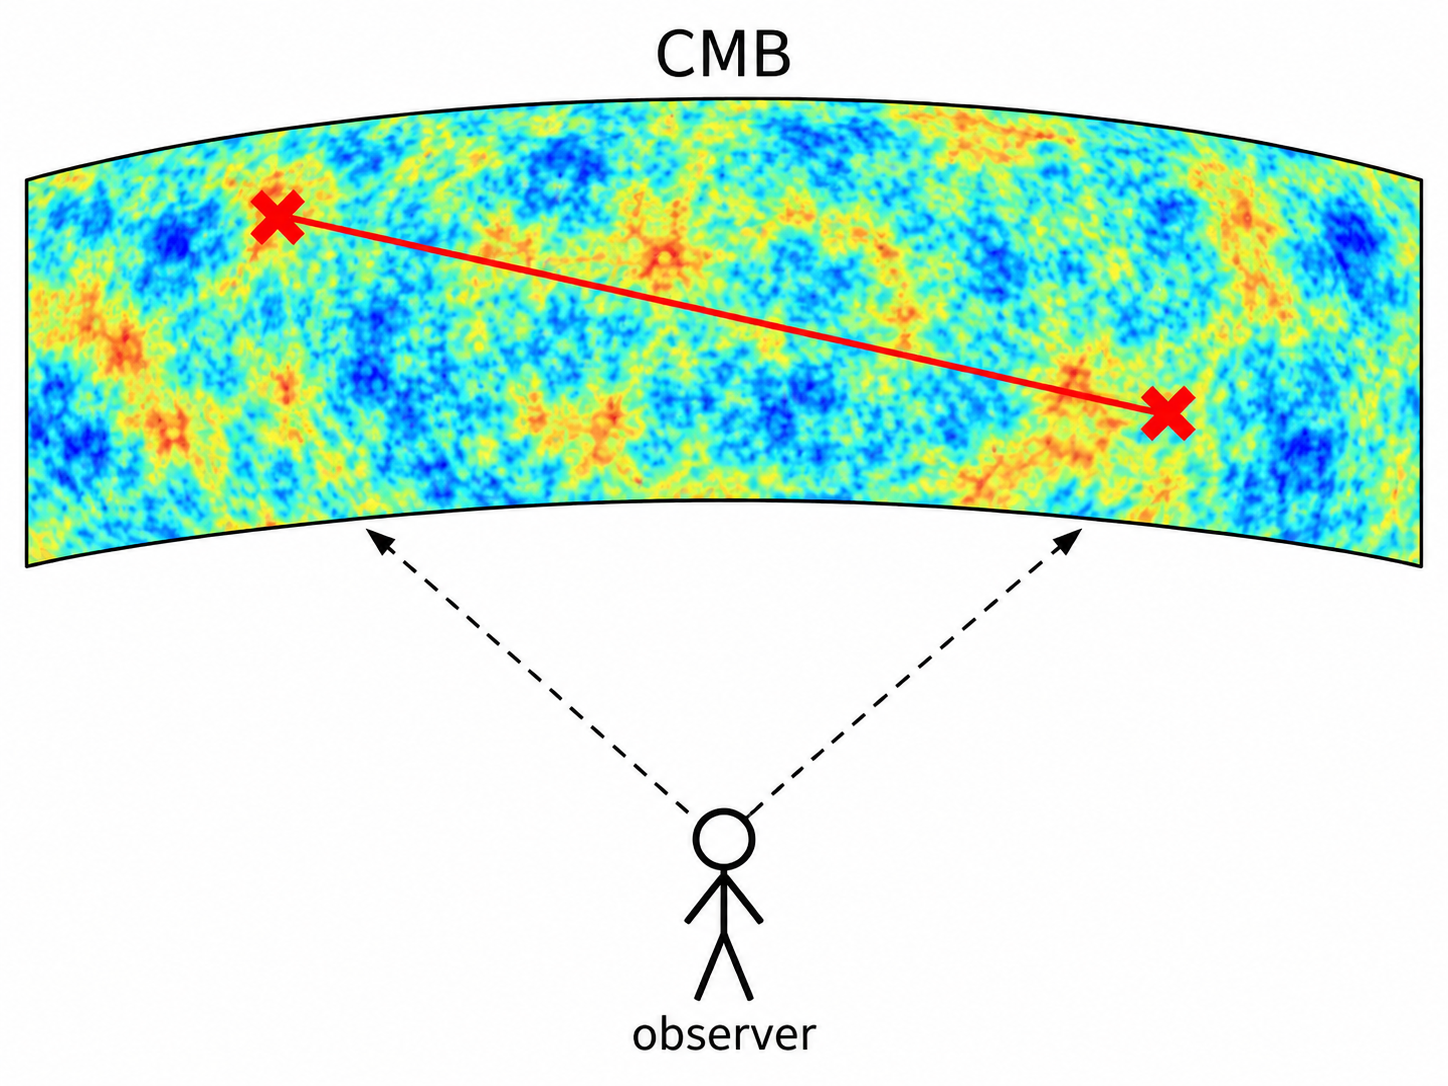
\includegraphics[width=0.7\textwidth]{Figures_Oral_CSI/observer.png}
		\end{figure}
		\end{column}
	\end{columns}
\end{frame}

\begin{frame}{Results: No-boundary vs Wineglass}
	\begin{columns}
		\begin{column}{0.7\textwidth}
			\begin{block}{}
				No-boundary proposal = pure de Sitter. Exact results are known for the \textit{Euclidean vacuum}.
		\begin{equation*}
			\langle |\Phi_{n \ell m}|^2 \rangle = \mathcal{P}_{N.B}(n; t=\infty) = \frac{H^2}{2n(n^2-1)}\,.
		\end{equation*}
			\end{block}
		\end{column}
		\begin{column}{0.29\textwidth}
			\begin{figure}[h!]
			\centering
			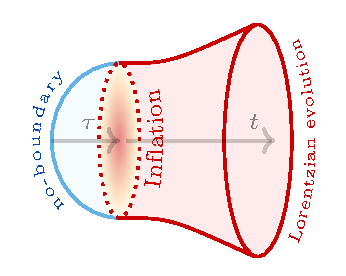
\includegraphics[width=0.7\textwidth]{Figures_Oral_CSI/singlenobound.pdf}
			\end{figure}
		\end{column}
	\end{columns}
	\pause
	\begin{columns}
		\begin{column}{0.49\textwidth}
		\begin{block}{}
			\begin{itemize}
				\item For the \textit{Wineglass Euclidean vacuum}, a WKB matching procedure at large $n$ gives
				\begin{equation*}
					\mathcal{P}_{WG}(n;t=\infty) \approx  \mathcal{P}_{N.B}(n; t=\infty)\,. 
				\end{equation*}
				\item Also, $\mathcal{P}_{WG}(1;t=\infty)<\infty$: boundary conditions break the shift symmetry.
			\end{itemize}
		\end{block}
		\end{column}
		\begin{column}{0.49\textwidth}
			\begin{figure}[h!]
			\centering
			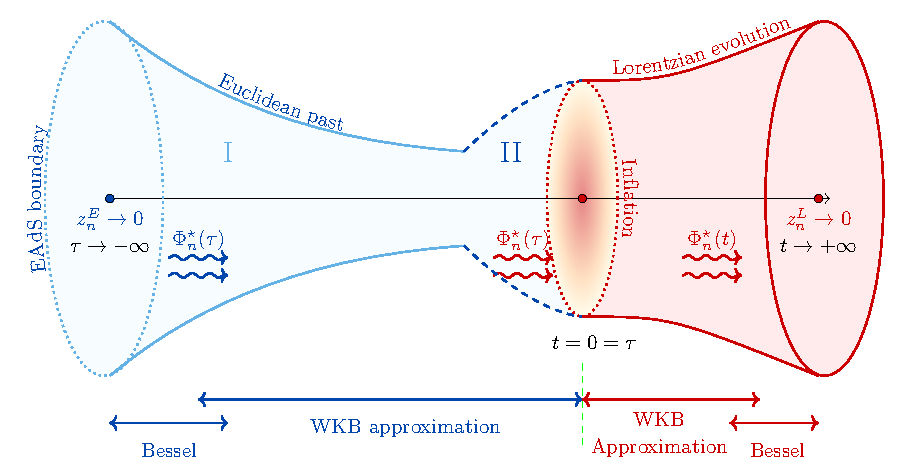
\includegraphics[width=1\textwidth]{Figures_Oral_CSI/WineglassBessel.pdf}
			\end{figure}
		\end{column}
	\end{columns}
\end{frame}
\begin{frame}{Numerical power spectrum}
  \begin{block}{Main conclusion}
    Wineglass corrections are confined to low harmonics; the spectrum rapidly approaches the Euclidean vacuum result at large $n$.
  \end{block}
  \begin{center}
    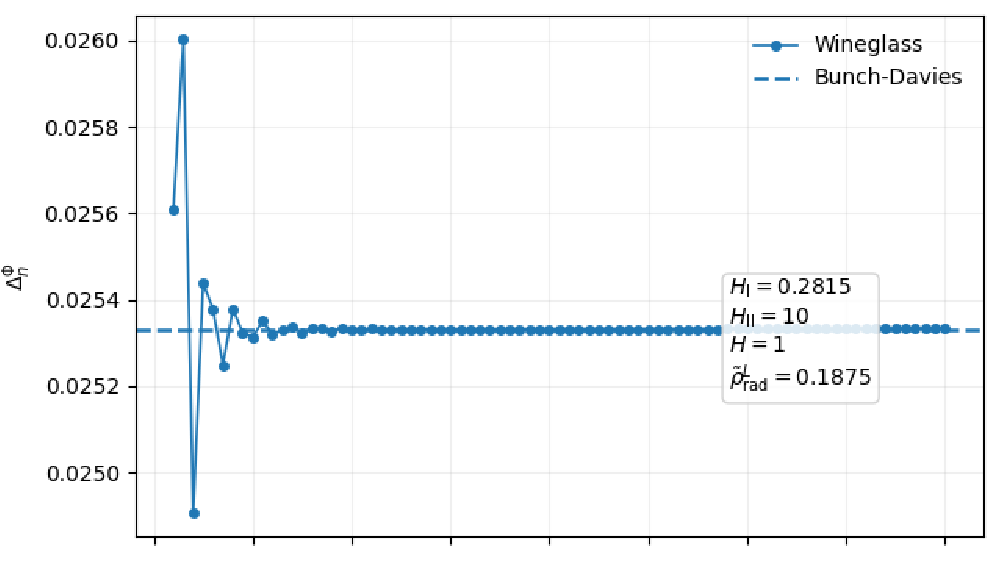
\includegraphics[width=0.5\textwidth]{Figures_Oral_CSI/newnew80harmonics_cropped.pdf}
  \end{center}
  \centering
  \small Dimensionless power spectrum:
  $\displaystyle \Delta_n=\frac{n(n^2-1)}{2\pi^2}\mathcal{P}(n;t=\infty)$.
\end{frame}

%======================================================================================================
\section{Boundary Liouville theory}
%======================================================================================================

\begin{frame}[plain]
  \centering
  {\Large\textbf{Part II --- Boundary Liouville theory}}\\[0.6cm]
  {\normalsize A complementary exactly solvable setting for quantum gravity}
\end{frame}

\begin{frame}{Bulk Liouville theory}
	\vspace{-0.5cm}
	\begin{block}{The action}
		\begin{equation*}
		\begin{aligned}
			\mathcal{S}_L &= \frac{1}{4\pi}\int \sqrt{\hat{g}}\, \rm{d}^2x\left(\hat{g}^{\mu \nu} \partial_\mu \phi \partial_\nu \phi + Q \hat{R}\phi + 4\pi \mu e^{2b\phi}\right)\, \quad \underset{\text{genus } 0}{\Rightarrow} \mathcal{S}_L = \frac{1}{4\pi}\int \rm{d}z \rm{d}\bar{z}(\partial_z\phi\partial_{\bar{z}}\phi+ 4\pi \mu e^{2b\phi})\\
			c &= 1+ 6Q^2 = 1 + 6(b+b^{-1})^2\,.
		\end{aligned}
		\end{equation*}
		$c\geq25, b \in (0,1] \Rightarrow$ "Spacelike" regime. 
		$c\leq1, \hat{b}=-ib \in (0,1] \Rightarrow$ "Timelike" regime.
	\end{block}
	\pause
	\begin{block}{Axiomatic bootstrap}
	Spectrum $\mathscr{H}$ is a rep of the Virasoro algebra closed under OPE. Commutativity of fields (in Euclidean). In Liouville field theory,
	\begin{itemize}
		\item Conformal dimensions $\Delta = \frac{c-1}{24}-P^2 \Rightarrow \mathscr{H} = \int_{i\mathbb{R}+(\epsilon)}^{\oplus} \rm{d}P\,\mathcal{V}_{P}\otimes \bar{\mathcal{V}}_{P} \Rightarrow$ \textbf{Continuous}.
		\item Spacelike Liouville is \textbf{unitary} but has no \textbf{vacuum} (and no degenerate rep in the spectrum)!
		\item Timelike Liouville is \textbf{non-unitary} but has a \textbf{vacuum} (and a degenerate rep in the spectrum)!
	\end{itemize}
	\end{block}
\end{frame}


\begin{frame}{Boundary Liouville bootstrap}
  \begin{block}{Add a boundary}
    \begin{equation*}
      \mathcal{S}_B=\mu_b\int_{\partial M}e^{b\phi}\,\mathrm{d}\xi,
      \qquad
      \mu_b^2=\frac{\mu\cosh^2(\pi\sigma/b)}{\sin(\pi b^2)}.
    \end{equation*}
    Boundary insertions introduce new CFT data.
  \end{block}
  \begin{columns}[T]
    \begin{column}{0.44\textwidth}
      \begin{block}{Known in the spacelike case}
        FZZT used bootstrap equations and Coulomb-gas/free-field techniques.
        \vspace{0.15cm}

        The analytic continuation to timelike Liouville is not straightforward.
      \end{block}
    \end{column}
    \begin{column}{0.54\textwidth}
      \begin{center}
        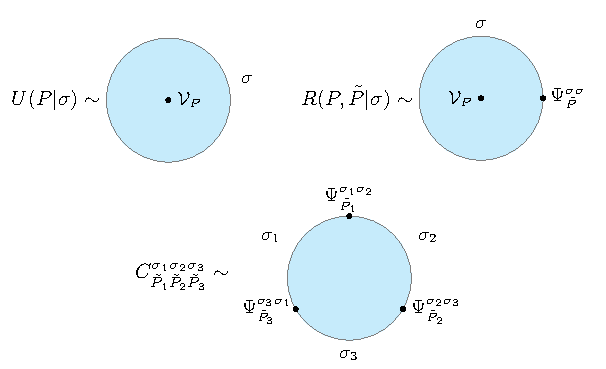
\includegraphics[width=0.92\textwidth]{Figures_Oral_CSI/CFTdata.pdf}
      \end{center}
    \end{column}
  \end{columns}
\end{frame}

\begin{frame}{Timelike case}
	\begin{block}{Strategy}
		\begin{itemize}
			\item [>] Merely a one-to-one correspondence between kernels and boundary CFT data \\
		$\Rightarrow$ Crossing equations = consistency conditions of the Moore-Seiberg groupoid.
			\item [>] Recent progress concerning the derivation of the kernels of timelike Liouville for $\hat{b}^2 \in \mathbb{Q}$ via Virasoro Wick rotation.
		\end{itemize}
	\end{block}
	\pause
	\begin{figure}[h!]
			\centering
			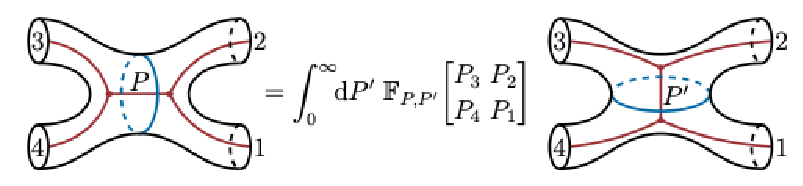
\includegraphics[width=0.5\textwidth]{Figures_Oral_CSI/Confblock.pdf}
	\end{figure}
	\begin{figure}[h!]
			\centering
			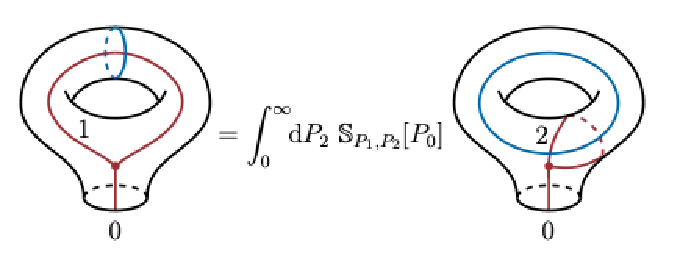
\includegraphics[width=0.5\textwidth]{Figures_Oral_CSI/Torrus.pdf}
	\end{figure}
\end{frame}

\begin{frame}{Relation between CFT data and kernels}
	\begin{columns}
		\begin{column}{0.49\textwidth}
			\begin{figure}[h!]
			\centering
			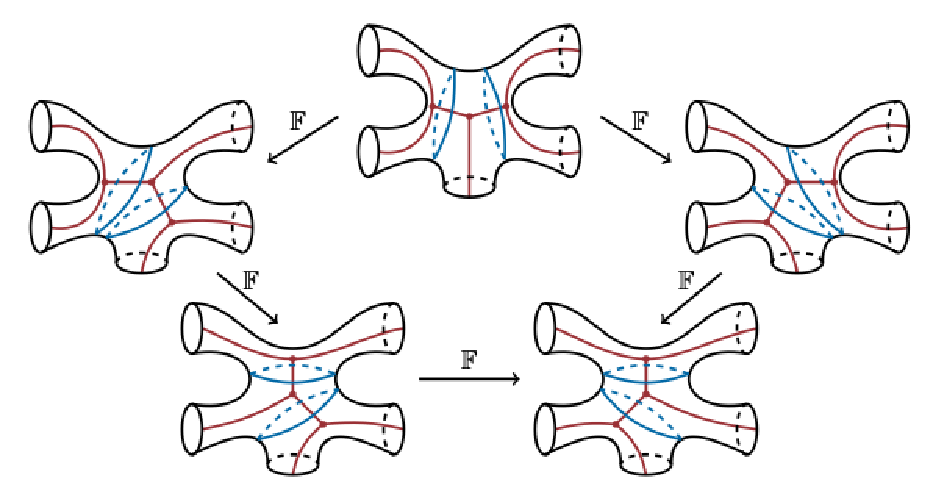
\includegraphics[width=0.5\textwidth]{Figures_Oral_CSI/Pentagon.pdf}
			\end{figure}
			\begin{figure}[h!]
			\centering
			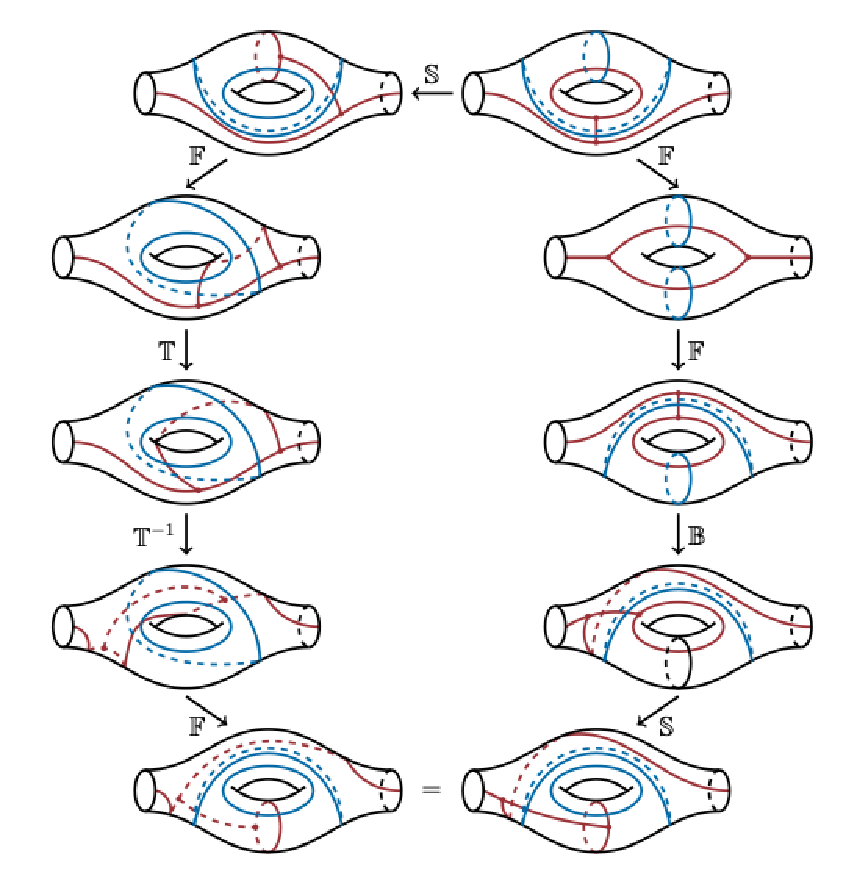
\includegraphics[width=0.5\textwidth]{Figures_Oral_CSI/2point.pdf}
			\end{figure}
		\end{column}
		\begin{column}{0.49\textwidth}
			\begin{block}{}
				\begin{equation*}
					\begin{aligned}
						\text{Pentagon equation} &\leftrightarrow \text{Crossing 4 pts bdy}\\
						\int \mathbb{F} \mathbb{F} \mathbb{F} = \mathbb{F} \mathbb{F} &\leftrightarrow \int C C \mathbb{F} = C C
					\end{aligned}
				\end{equation*}

				\begin{equation*}
					\begin{aligned}
						\text{Torus 2 pt} \leftrightarrow &\text{ 2 bulk and 1 bdy crossing}\\
						\mathbb{S} \mathbb{F} = \int \int e^{i \theta} \mathbb{S} \mathbb{F}  \mathbb{F}  \mathbb{F} &\leftrightarrow R C  = \int \int e^{i \theta} R C \mathbb{F} \mathbb{F}
					\end{aligned}
				\end{equation*}
			\end{block}
			\begin{block}{}
				\begin{itemize}
					\item [>] In the spacelike case, this gives $C \propto \mathbb{F},\,R \propto \mathbb{S}$ with $\mathbb{F}$ and $\mathbb{S}$ known.
					\item [>] In the timelike case, it remains to find kernels solving the consistency relations.
				\end{itemize}
			\end{block}
		\end{column}
	\end{columns}
\end{frame}

\begin{frame}{Preliminary timelike results}
  \begin{block}{Working at rational $\hat b^2$}
    \begin{itemize}
      \item The shift equations admit a two-dimensional vector space of kernel solutions.
      \item The physical kernel solving four-point crossing is non-meromorphic.
      \item The candidate CFT data are associated with the meromorphic Virasoro-Wick-rotated kernels.
    \end{itemize}
  \end{block}
  \begin{block}{Conjectural identification}
    \begin{equation*}
      C\propto\mathcal{R}\mathbb{F},
      \qquad
      R\propto\mathcal{R}\mathbb{S}.
    \end{equation*}
    Numerical evidence and analytic arguments support this construction, with evidence for uniqueness for $c\leq1$.
  \end{block}
\end{frame}

\begin{frame}{Conclusions and next steps}
  \begin{block}{Wineglass cosmology}
    Phase diagram completed; next step: finish the power spectrum analysis and sharpen the WKB matching argument.
  \end{block}
  \begin{block}{Boundary timelike Liouville}
    Candidate boundary CFT data from Virasoro-Wick-rotated kernels. Next step: write down the analytic derivation and produce precise numerical plots showing evidence for the conjecture.
  \end{block}
  \begin{block}{Other directions}
    Entanglement entropy in $c=1$ MQM; axion wormholes and dynamical-systems methods.
  \end{block}
  \centering
  \textbf{Near-term objective: complete the ongoing projects/prepare the corresponding papers/present the works next year.}
\end{frame}

\end{document}
